\documentclass[11pt]{article}

\usepackage[T1]{fontenc}
\usepackage{amsmath,amssymb,amsthm}
\usepackage{graphicx}
\usepackage{geometry}
\usepackage[colorlinks=true,linkcolor=blue,citecolor=blue,urlcolor=blue]{hyperref}
\geometry{margin=1in}

\newtheorem{theorem}{Theorem}
\newtheorem{corollary}{Corollary}

\newcommand{\R}{\mathbb R}
\newcommand{\E}{\mathbb E}
\newcommand{\supp}{\operatorname{supp}}

\title{A \(p>2\) obstruction for the restricted isomorphism property into \(\ell_r\)}
\author{Run fa\_banach\_001, agent lane 13}
\date{2026-06-19}

\begin{document}
\maketitle

\begin{abstract}
Friedland and Guedon ask what happens for \(p>2\) in their search for
operators satisfying the restricted isomorphism property \(\mathcal P_1(m)\).
Their \(0<p<2\) construction uses \(p\)-stable random variables and yields
large sparsity order for operators into \(\ell_r^N\), \(0<r\le1\).  We prove
that this target family has a simple obstruction when \(p>2\): if
\(A:\ell_p^n\to\ell_r^N\), \(0<r\le1\), satisfies \(\mathcal P_1(m)\) with
distortion \(\beta/\alpha\), then
\[
  m^{1/2-1/p}\lesssim_r \beta/\alpha.
\]
Thus fixed-distortion \(\ell_r\)-valued restricted isomorphisms cannot have
sparsity order \(m\to\infty\) for \(p>2\).  This bound is sharp: normalized
Gaussian maps into \(\ell_r^N\), \(N\gtrsim_r m\log(en/m)\), satisfy
\(\mathcal P_1(m)\) with distortion \(\lesssim_r m^{1/2-1/p}\).  The same
lower-bound proof gives an analogous cotype-2 obstruction for Banach targets
such as Hilbert spaces and \(L_1\).
\end{abstract}

\section{Source question}

The source defines \(\operatorname{sparse}(m)=\{x\in\R^n:|\supp x|\le m\}\).
An operator \(A:\ell_p^n\to E_1\) satisfies property \(\mathcal P_1(m)\) if
there are constants \(\alpha,\beta>0\) such that
\[
  \forall x\in\operatorname{sparse}(m)\qquad
  \alpha |x|_p\le \|Ax\|_{E_1}\le \beta |x|_p.
\]

\begin{figure}[h]
\centering
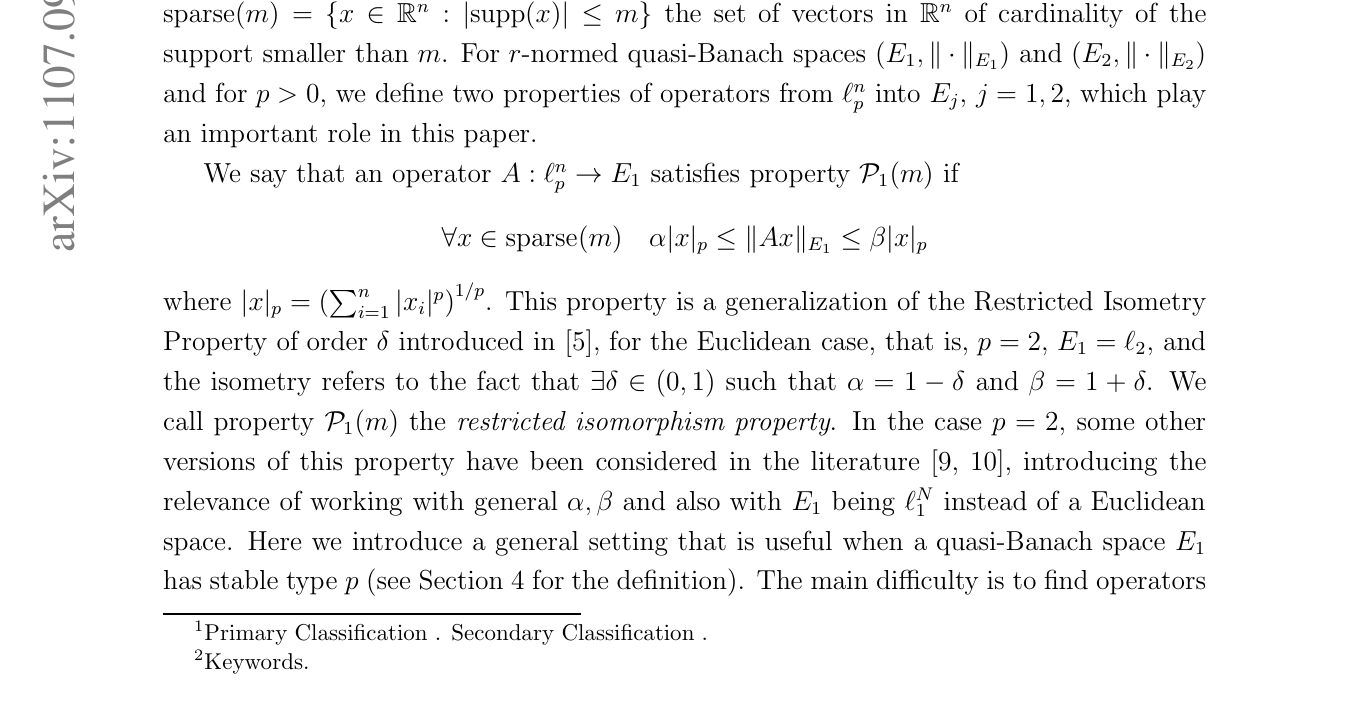
\includegraphics[width=.95\textwidth]{figures/p1_definition_crop.png}
\caption{The source definition of \(\mathcal P_1(m)\).}
\end{figure}

After recalling that many random matrices satisfy this property for \(p=2\),
and after announcing a \(p\)-stable construction for \(0<p<2\), the source
asks what happens for \(p>2\):

\begin{figure}[h]
\centering
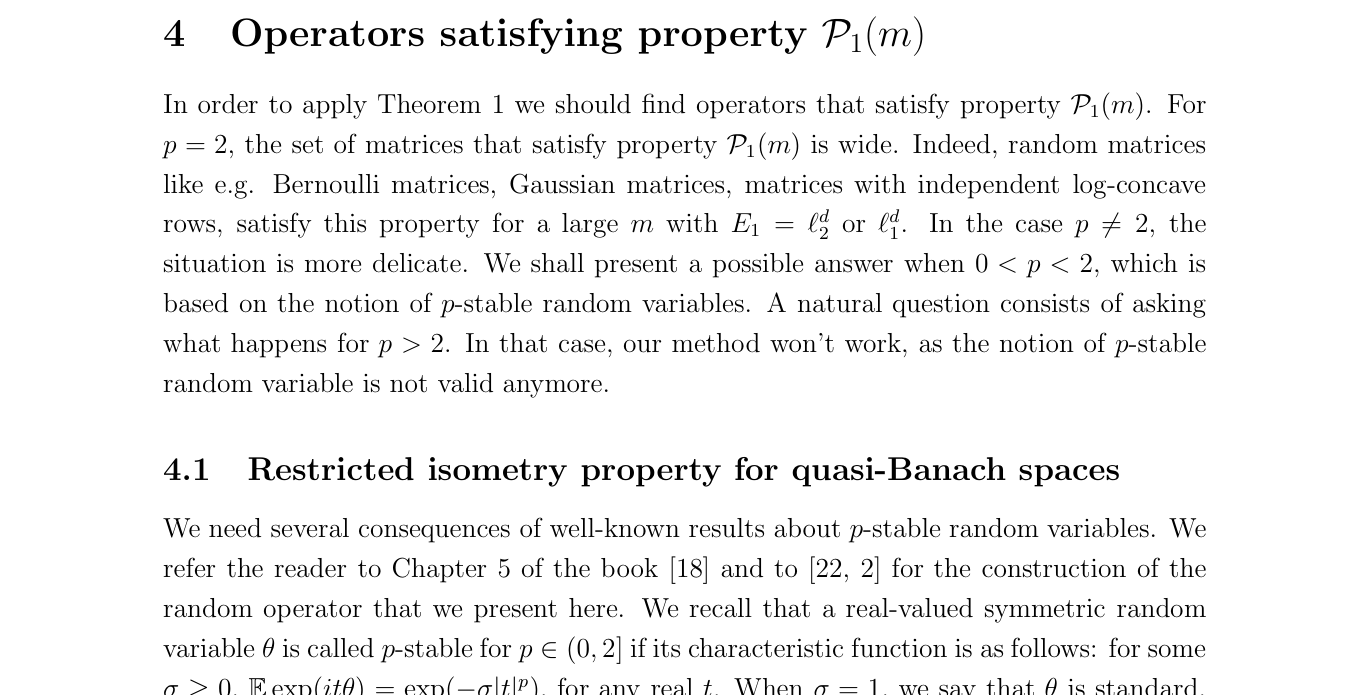
\includegraphics[width=.95\textwidth]{figures/p_gt_2_question_crop.png}
\caption{The source paragraph asking about \(p>2\).}
\end{figure}

\section{The obstruction}

\begin{theorem}\label{thm:lr}
Let \(p>2\), \(0<r\le1\), and \(1\le m\le n\).  Suppose that
\[
  A:\ell_p^n\longrightarrow \ell_r^N
\]
satisfies \(\mathcal P_1(m)\) with constants \(\alpha,\beta>0\), where
\(\ell_r^N\) is equipped with the usual quasi-norm
\(\|z\|_r=(\sum_{j=1}^N |z_j|^r)^{1/r}\).  Then
\[
  m^{1/2-1/p}\le K_r\,\frac{\beta}{\alpha},
\]
where \(K_r\) depends only on \(r\).  Consequently, for fixed \(p>2\), \(r\),
and fixed distortion \(\beta/\alpha\), the order \(m\) is bounded independently
of \(n\) and \(N\).
\end{theorem}

\begin{proof}
Fix a coordinate set \(I\subset\{1,\ldots,n\}\) with \(|I|=m\), and write
\(y_i=Ae_i\in\ell_r^N\) for \(i\in I\).  Since each \(e_i\) is
\(m\)-sparse,
\[
  \|y_i\|_r\ge \alpha,\qquad i\in I.
\]
Also, for every choice of signs \(\varepsilon_i\in\{-1,1\}\),
\[
  \left\|\sum_{i\in I}\varepsilon_i y_i\right\|_r
  \le \beta \left|\sum_{i\in I}\varepsilon_i e_i\right|_p
  = \beta m^{1/p}.
\]

Let \((\varepsilon_i)_{i\in I}\) be independent Rademacher signs.  The lower
Khinchine inequality says that for every scalar family \((a_i)_{i\in I}\),
\[
  \E\left|\sum_{i\in I}\varepsilon_i a_i\right|^r
  \ge k_r\left(\sum_{i\in I}|a_i|^2\right)^{r/2}
\]
with \(k_r>0\) depending only on \(r\).  Applying this coordinatewise gives
\[
\begin{aligned}
  \beta^r m^{r/p}
  &\ge
  \E\left\|\sum_{i\in I}\varepsilon_i y_i\right\|_r^r  \\
  &= \sum_{j=1}^N
     \E\left|\sum_{i\in I}\varepsilon_i y_i(j)\right|^r \\
  &\ge
     k_r\sum_{j=1}^N
       \left(\sum_{i\in I}|y_i(j)|^2\right)^{r/2}.
\end{aligned}
\]
For \(0<r\le1\), and hence \(r\le2\), the elementary power-mean inequality
gives, for each \(j\),
\[
  \left(\sum_{i\in I}|y_i(j)|^2\right)^{r/2}
  \ge m^{r/2-1}\sum_{i\in I}|y_i(j)|^r.
\]
Therefore
\[
\begin{aligned}
  \beta^r m^{r/p}
  &\ge k_r m^{r/2-1}
       \sum_{i\in I}\sum_{j=1}^N |y_i(j)|^r  \\
  &= k_r m^{r/2-1}\sum_{i\in I}\|y_i\|_r^r
   \ge k_r \alpha^r m^{r/2}.
\end{aligned}
\]
Taking \(r\)-th roots yields
\[
  m^{1/2-1/p}\le k_r^{-1/r}\,\frac{\beta}{\alpha}.
\]
This is the desired estimate, with \(K_r=k_r^{-1/r}\).
\end{proof}

\section{Sharpness for \texorpdfstring{\(\ell_r\)}{ell-r}-valued maps}

\begin{theorem}\label{thm:upper}
Let \(p>2\), \(0<r\le1\), and \(1\le m\le n\).  For every
\(0<\delta<1\), if
\[
  N\ge C_r\delta^{-2}m\log(en/m),
\]
then with positive probability the Gaussian operator
\[
  A x=\mu_r^{-1/r}N^{-1/r}\big(\langle g_1,x\rangle,\ldots,
  \langle g_N,x\rangle\big),\qquad
  \mu_r=\E |g|^r,
\]
where \(g_1,\ldots,g_N\) are independent standard Gaussian vectors in
\(\R^n\), satisfies
\[
  (1-\delta)|x|_2\le \|Ax\|_r\le(1+\delta)|x|_2
\]
for every \(m\)-sparse \(x\in\R^n\).  Consequently, as an operator
\(\ell_p^n\to\ell_r^N\), it satisfies \(\mathcal P_1(m)\) with
\[
  \alpha=1-\delta,\qquad
  \beta=(1+\delta)m^{1/2-1/p}.
\]
\end{theorem}

\begin{proof}
We use the standard Gaussian restricted-isometry net argument, adapted to the
\(\ell_r\) quasi-norm.  For a fixed Euclidean unit vector \(x\), the random
variables \(|\langle g_j,x\rangle|^r\) are independent copies of \(|g|^r\).
Since \(|g|^r\) has sub-exponential tails for \(0<r\le1\), Bernstein's
inequality gives constants \(c_r,C_r>0\) such that
\[
 \Pr\left\{\left|N^{-1}\sum_{j=1}^N|\langle g_j,x\rangle|^r-\mu_r\right|
       >\varepsilon\mu_r\right\}
 \le 2e^{-c_r\varepsilon^2N},\qquad 0<\varepsilon<1.
\]

Fix a support \(I\subset\{1,\ldots,n\}\), \(|I|=m\), and take an
\(\eta\)-net \(\mathcal N_I\) of the Euclidean unit sphere in \(\R^I\) with
\(|\mathcal N_I|\le (1+2/\eta)^m\).  A union bound over all supports and all
net points shows that, provided
\[
 N\ge C_r\varepsilon^{-2}m\log(en/m),
\]
we have, with positive probability,
\[
  (1-\varepsilon)\mu_r
  \le N^{-1}\sum_{j=1}^N|\langle g_j,y\rangle|^r
  \le (1+\varepsilon)\mu_r
\]
simultaneously for every \(y\in\bigcup_I\mathcal N_I\).

On this event, pass from the net to the full sparse Euclidean sphere.  For a
fixed support \(I\), put
\[
  M_I=\sup\{\|Ax\|_r^r: x\in\R^I,\ |x|_2=1\}.
\]
If \(x\) is in that sphere and \(y\in\mathcal N_I\) satisfies
\(|x-y|_2\le\eta\), the \(r\)-triangle inequality gives
\[
  \|Ax\|_r^r\le \|Ay\|_r^r+\|A(x-y)\|_r^r
  \le (1+\varepsilon)^r+\eta^r M_I.
\]
Thus \(M_I\le (1+\varepsilon)^r/(1-\eta^r)\).  The reverse estimate follows
from
\[
  \|Ax\|_r^r\ge \|Ay\|_r^r-\|A(x-y)\|_r^r
  \ge (1-\varepsilon)^r-\eta^r M_I.
\]
Choosing \(\eta,\varepsilon\) as sufficiently small constant multiples of
\(\delta\), with constants depending only on \(r\), yields the stated
\((1\pm\delta)\) estimate after the normalization by \(\mu_r^{-1/r}N^{-1/r}\).

Finally, for \(m\)-sparse \(x\) and \(p>2\),
\[
  |x|_p\le |x|_2\le m^{1/2-1/p}|x|_p.
\]
Combining this with the Euclidean estimate gives \(\mathcal P_1(m)\) with the
displayed constants.
\end{proof}

\begin{corollary}\label{cor:cotype}
Let \(p>2\), and let \(E\) be a Banach space with cotype \(2\) constant
\(C_2(E)\).  If \(A:\ell_p^n\to E\) satisfies \(\mathcal P_1(m)\) with
constants \(\alpha,\beta\), then
\[
  m^{1/2-1/p}\le C_2(E)\,\frac{\beta}{\alpha}.
\]
\end{corollary}

\begin{proof}
With \(y_i=Ae_i\) as above, the lower part of \(\mathcal P_1(m)\) gives
\((\sum_{i\in I}\|y_i\|^2)^{1/2}\ge \alpha m^{1/2}\).  By cotype \(2\),
\[
  \alpha m^{1/2}
  \le C_2(E)\left(\E\left\|\sum_{i\in I}\varepsilon_i y_i\right\|^2\right)^{1/2}.
\]
The upper part of \(\mathcal P_1(m)\), applied to all signed sums, bounds the
last factor by \(\beta m^{1/p}\).
\end{proof}

\section{Interpretation}

The source's \(0<p<2\) construction obtains \(m\) proportional to
\(\eta n/\log(1+1/\eta)\) for operators into \(\ell_r^{\eta n}\), \(0<r\le1\).
Theorem \ref{thm:lr} shows that no analogous result can hold for \(p>2\) with
the same target family and fixed distortion.  This is independent of the
random model: it excludes every linear operator \(A:\ell_p^n\to\ell_r^N\).
Theorem \ref{thm:upper} shows that the obstruction is the right one: the best
possible \(p>2\) behavior for \(\ell_r\)-targets is the Euclidean sparse
behavior, with unavoidable distortion of order \(m^{1/2-1/p}\).

Corollary \ref{cor:cotype} also explains why the Hilbert and \(\ell_1^N\)
targets mentioned in the \(p=2\) discussion cannot support a large-order
\(\mathcal P_1(m)\) theory for \(p>2\) with uniform constants.  Hilbert spaces
and \(L_1\)-spaces have cotype \(2\) with universal constants.

This is a partial answer only.  It does not rule out all possible quasi-Banach
targets for \(p>2\); it rules out the paper's natural \(\ell_r\)-target
extension with fixed distortion, gives the sharp distortion tradeoff for
\(\ell_r\)-targets, and rules out the standard Banach targets of cotype \(2\)
when one asks for large \(m\) with uniform constants.

\section{Novelty check}

The run indexes were searched for arXiv:1107.0992, the title, restricted
isomorphism property, \(p>2\), sparsity, and related embedding keywords.  No
prior packet was found.  Web searches on 2026-06-19 for the exact title with
``\(p>2\)'', for ``property \(P_1(m)\) \(p>2\)'', and for restricted
isomorphism property of \(\ell_p\) into \(\ell_r\) found the source paper but
no later exact answer to this \(p>2\) gap.

\begin{thebibliography}{9}

\bibitem{FG}
Omer Friedland and Olivier Guedon,
\emph{Sparsity and non-Euclidean embeddings},
arXiv:1107.0992, 2011.
\url{https://arxiv.org/abs/1107.0992}

\bibitem{LT}
Michel Ledoux and Michel Talagrand,
\emph{Probability in Banach Spaces: Isoperimetry and Processes},
Springer, 1991.

\bibitem{FR}
Simon Foucart and Holger Rauhut,
\emph{A Mathematical Introduction to Compressive Sensing},
Birkhauser, 2013.

\end{thebibliography}

\end{document}
